%\chapter{Background}  \label{background}
\chapter{Background}  \label{background}
A programming language is described by the combination of its syntax and semantics. The syntax concerns the legal structures of programs written in the programming language, while the semantics is about the meaning of every construct in that language. Furthermore, the abstract syntactic structure of source code written in a programming language can be represented as an \emph{abstract syntax tree} (AST), in which nodes are occurrences of syntactic structures and edges represent nesting relationships. Since ASTs will be the form in which I represent and analyze source code, I need a means to generalize sets of ASTs in order to understand their commonalities while abstracting away their differences. The theoretical framework of anti-unification is presented as that means.

In this chapter, ASTs are described in Section~\ref{AST}, along with their more concrete counterparts, concrete syntax trees. A specific, industrial framework for creating and manipulating ASTs for source code written in the Java programming language---the Eclipse JDT---is described in Section~\ref{JDT}.  Anti-unification is summarized in Section~\ref{AU}, starting with its most basic form, first-order anti-unification, and progressing to the form that I will make use of, higher-order anti-unification modulo equational theories, in Section~\ref{HOAUMT}.  A research approach, built atop the Eclipse JDT, for performing anti-unification on Java ASTs---the Jigsaw framework---is described in Section~\ref{Jigsaw}. In the last section of this chapter, I provide some background information about clustering, existing clustering techniques, and the agglomerative hierarchical clustering algorithm, as a technique I used to cluster logged methods into separate groups based on a similarity measurement.
%AHC???
% as a technique or the technique??

\section{Concrete syntax trees and abstract syntax trees}\label{AST}

A concrete syntax tree is a tree $T=(V,E)$ whose vertices $V$ (equivalently, nodes) represent the syntactic structures (equivalently, syntactic elements) of a specific program written in a specific programming language and whose directed edges $E$ represent the nesting relationships amongst those syntactic structures.  Non-leaf nodes in a concrete syntax tree (also called a parse tree) represent the grammar productions that were satisfied in parsing the program it represents; leaf nodes represent the concrete lexemes, such as literals and keywords.

I focus on the Java programming language and I make use of the grammar in the language specification \cite[][Chapter 18]{2012:book:gosling} to determine the form of the concrete syntax trees.  Non-leaf node names are represented by names in ``camel-case'' written in italics.  Consider the trivial program in Figure~\ref{fig:java-example}; its concrete syntax tree is represented in Figure~\ref{fig:java-example-cst}.

\begin{figure}
\begin{lstlisting}
public class HelloWorld {
    public static void main(String[] args) {
        System.out.println("Hello world!");
    }
}
\end{lstlisting}
\caption{A simple example Java program.\label{fig:java-example}}
\end{figure}

\begin{sidewaysfigure}
\centering\resizebox{!}{0.65\textheight}{%
\begin{tikzpicture}
\node(cu) at (-14,20) {\textit{compilationUnit}};
%
\node(td) at (-14,19) {\textit{typeDeclaration}};
\draw[->](cu) -- (td) {};
%
\node(cid) at (-14,18) {\textit{classOrInterfaceDeclaration}};
\draw[->](td) -- (cid) {};
%
\node(mod2) at (-16,17) {\textit{modifier}};
\draw[->](cid) -- (mod2) {};
%
\node(public2) at (-16,16) {\textsf{\small public}};
\draw[->](mod2) -- (public2) {};
%
\node(cd) at (-12,17) {\textit{classDeclaration}};
\draw[->](cid) -- (cd) {};
%
\node(ncd) at (-12,16) {\textit{normalClassDeclaration}};
\draw[->](cd) -- (ncd) {};
%
\node(class) at (-16,15) {\textsf{\small class}};
\node(id7) at (-14,15) {\textit{identifier}};
\node(cbody) at (-8,15) {\textit{classBody}};
\draw[->](ncd) -- (class) {};
\draw[->](ncd) -- (id7) {};
\draw[->](ncd) -- (cbody) {};
%
\node(HelloWorld) at (-14,14) {\textsf{\small HelloWorld}};
\draw[->](id7) -- (HelloWorld) {};
%
\node(obr2) at (-12,14) {\textsf{\small \{}};
\node(cbd) at (-8,14) {\textit{classBodyDeclaration}};
\node(cbr2) at (-4,14) {\textsf{\small \}}};
\draw[->](cbody) -- (obr2) {};
\draw[->](cbody) -- (cbd) {};
\draw[->](cbody) -- (cbr2) {};
%
\node(mod1) at (-12,13) {\textit{modifier}};
\node(mod2) at (-10,13) {\textit{modifier}};
\node(md) at (-4,13) {\textit{memberDecl}};
\draw[->](cbd) -- (mod1) {};
\draw[->](cbd) -- (mod2) {};
\draw[->](cbd) -- (md) {};
%
\node(public1) at (-12,12) {\textsf{\small public}};
\draw[->](mod1) -- (public1) {};
%
\node(static) at (-10,12) {\textsf{\small static}};
\draw[->](mod2) -- (static) {};
%
\node(void) at (-8,12) {\textsf{\small void}};
\node(id6) at (-6,12) {\textit{identifier}};
\node(vmdr) at (2,12) {\textit{voidMethodDeclaratorRest}};
\draw[->](md) -- (void) {};
\draw[->](md) -- (id6) {};
\draw[->](md) -- (vmdr) {};
%
\node(main) at (-6,11) {\textsf{\small main}};
\draw[->](id6) -- (main) {};
%
\node(formals) at (-2,11) {\textit{formalParameters}};
\draw[->](vmdr) -- (formals) {};
%
\node(op2) at (-5,10) {\textsf{\small (}};
\node(fpd) at (-2,10) {\textit{formalParameterDecls}};
\node(cp2) at (1,10) {\textsf{\small )}};
\draw[->](formals) -- (op2) {};
\draw[->](formals) -- (fpd) {};
\draw[->](formals) -- (cp2) {};
%
\node(type) at (-4,9) {\textit{type}};
\node(fpdr) at (0,9) {\textit{formalParameterDeclsRest}};
\draw[->](fpd) -- (type) {};
\draw[->](fpd) -- (fpdr) {};
%
\node(rt) at (-6,8) {\textit{referenceType}};
\node(obt) at (-4,8) {\textsf{\small [}};
\node(cbt) at (-3,8) {\textsf{\small ]}};
\draw[->](type) -- (rt) {};
\draw[->](type) -- (obt) {};
\draw[->](type) -- (cbt) {};
%
\node(id5) at (-6,7) {\textit{identifier}};
\draw[->](rt) -- (id5) {};
%
\node(String) at (-6,6) {\textsf{\small String}};
\draw[->](rt) -- (String) {};
%
\node(vdi) at (0,8) {\textit{variableDeclaratorId}};
\draw[->](fpdr) -- (vdi) {};
%
\node(id4) at (0,7) {\textit{identifier}};
\draw[->](vdi) -- (id4) {};
%
\node(args) at (0,6) {\textsf{\small args}};
\draw[->](id4) -- (args) {};
%
\node(block) at (6,11) {\textit{block}};
\draw[->](vmdr) -- (block) {};
%
\node(obrace1) at (4,10) {\textsf{\small \{}};
\node(bs1) at (6,10) {\textit{blockStatements}};
\node(cbrace1) at (8,10) {\textsf{\small \}}};
\draw[->](block) -- (obrace1) {};
\draw[->](block) -- (bs1) {};
\draw[->](block) -- (cbrace1) {};
%
\node(bs2) at (6,9) {\textit{blockStatement}};
\draw[->](bs1) -- (bs2) {};
%
\node(stat) at (6,8) {\textit{statement}};
\draw[->](bs2) -- (stat) {};
%
\node(se) at (5,7) {\textit{statementExpression}};
\node(sc) at (7.5,7) {\textsf{\small ;}};
\draw[->](stat) -- (se) {};
\draw[->](stat) -- (sc) {};
%
\node(expr) at (5,6) {\textit{expression}};
\draw[->](se) -- (expr) {};
%
\node(e1) at (5,5) {\textit{expression1}};
\draw[->](expr) -- (e1) {};
%
\node(e2) at (5,4) {\textit{expression2}};
\draw[->](e1) -- (e2) {};
%
\node(e3) at (5,3) {\textit{expression3}};
\draw[->](e2) -- (e3) {};
%
\node(prim1) at (2,2) {\textit{primary}};
\node(sel) at (8,2) {\textit{selector}};
\draw[->](e3) -- (prim1) {};
\draw[->](e3) -- (sel) {};
%
\node(id1) at (0,1) {\textit{identifier}};
\node(dot1) at (2,1) {\textsf{\small .}};
\node(id2) at (4,1) {\textit{identifier}};
\draw[->](prim1) -- (id1) {};
\draw[->](prim1) -- (dot1) {};
\draw[->](prim1) -- (id2) {};
%
\node(dot2) at (6,1) {\textsf{\small .}};
\node(id3) at (8,1) {\textit{identifier}};
\node(arguments) at (11,1) {\textit{arguments}};
\draw[->](sel) -- (dot2) {};
\draw[->](sel) -- (id3) {};
\draw[->](sel) -- (arguments) {};
%
\node(System) at (0,0) {\textsf{\small System}};
\draw[->](id1) -- (System) {};
%
\node(out) at (4,0) {\textsf{\small out}};
\draw[->](id2) -- (out) {};
%
\node(println) at (8,0) {\textsf{\small println}};
\draw[->](id3) -- (println) {};
%
\node(op) at (9,0) {\textsf{\small (}};
\node(sl) at (11,0) {\textsf{\small "Hello world!"}};
\node(cp) at (13,0) {\textsf{\small )}};
\draw[->](arguments) -- (op) {};
\draw[->](arguments) -- (sl) {};
\draw[->](arguments) -- (cp) {};
\end{tikzpicture}%
}
\caption{The concrete syntax tree for the program of Figure~\ref{fig:java-example}.\label{fig:java-example-cst}}
\end{sidewaysfigure}

Beyond the fact that the concrete syntax tree is rather verbose and thus occupies a lot of space even for a trivial example, I can see two key problems with it: (1)~there are a multitude of redundant nodes such as \textit{expression1}, \textit{expression2}, and \textit{expression3} that are present solely for purposes of creating an unambiguous grammar; and (2)~there are no nodes that express key concepts, such as ``method declaration'' and ``method invocation'', that should be obviously present in the example program.

To address these problems, concrete syntax trees are converted to abstract syntax trees (ASTs). An AST is similar in concept to a concrete syntax tree but it does not generally represent the parsing steps followed to differentiate different kinds of syntactic structure. The node types are chosen to represent syntactical concepts; I use the grammar presented for exposition by \citet{2012:book:gosling}, which differs markedly from the grammar they propose in their Chapter~18 for efficient parsing. Note that a given node type constrains the kinds and numbers of child nodes that it possesses. The AST derived from the concrete syntax tree of Figure~\ref{fig:java-example-cst} is shown in Figure~\ref{fig:java-example-ast}. Note that, although I know that (for any normal program) \code{System} refers to the class \code{java.lang.System} and \code{out} is a static field on that class, non-normal programs can occur and a pure syntactic analysis cannot rule out that \code{System} is a package and that \code{out} is a class therein declaring a static method \code{println(String)}.

\begin{sidewaysfigure}
\centering\resizebox{!}{0.4\textheight}{%
\begin{tikzpicture}
\node(cu) at (-12,11) {\textit{compilationUnit}};
%
\node(cd) at (-12,10) {\textit{classDeclaration}};
\draw[->](cu) -- (cd) {};
%
\node(mod3) at (-16,9) {\textit{modifier}};
\node(class) at (-14,9) {\textsf{\small class}};
\node(id7) at (-12,9) {\textit{identifier}};
\node(cbody) at (-4,9) {\textit{classBody}};
\draw[->](cd) -- (mod3) {};
\draw[->](cd) -- (class) {};
\draw[->](cd) -- (id7) {};
\draw[->](cd) -- (cbody) {};
%
\node(public2) at (-16,8) {\textsf{\small public}};
\draw[->](mod3) -- (public2) {};
%
\node(HelloWorld) at (-12,8) {\textsf{\small HelloWorld}};
\draw[->](id7) -- (HelloWorld) {};
%
\node(obr2) at (-8,8) {\textsf{\small \{}};
\node(md) at (-4,8) {\textit{methodDeclaration}};
\node(cbr2) at (0,8) {\textsf{\small \}}};
\draw[->](cbody) -- (obr2) {};
\draw[->](cbody) -- (md) {};
\draw[->](cbody) -- (cbr2) {};
%
\node(mod1) at (-12,6) {\textit{modifier}};
\node(mod2) at (-10,6) {\textit{modifier}};
\node(result) at (-8,6) {\textit{result}};
\node(id6) at (-6,6) {\textit{identifier}};
\node(fps) at (-2,6) {\textit{formalParameters}};
\node(mbody) at (6,6) {\textit{methodBody}};
\draw[->](md) -- (mod1) {};
\draw[->](md) -- (mod2) {};
\draw[->](md) -- (result) {};
\draw[->](md) -- (id6) {};
\draw[->](md) -- (fps) {};
\draw[->](md) -- (mbody) {};
%
\node(public1) at (-12,5) {\textsf{\small public}};
\draw[->](mod1) -- (public1) {};
%
\node(static) at (-10,5) {\textsf{\small static}};
\draw[->](mod2) -- (static) {};
%
\node(void) at (-8,5) {\textsf{\small void}};
\draw[->](result) -- (void) {};
%
\node(main) at (-6,5) {\textsf{\small main}};
\draw[->](id6) -- (main) {};
%
\node(op2) at (-4,5) {\textsf{\small (}};
\node(fp) at (-2,5) {\textit{formalParameter}};
\node(cp2) at (0,5) {\textsf{\small )}};
\draw[->](fps) -- (op2) {};
\draw[->](fps) -- (fp) {};
\draw[->](fps) -- (cp2) {};
%
\node(type) at (-4,4) {\textit{arrayType}};
\node(id5) at (0,4) {\textit{identifier}};
\draw[->](fp) -- (type) {};
\draw[->](fp) -- (id5) {};
%
\node(id4) at (-6,3) {\textit{identifier}};
\node(obt) at (-4,3) {\textsf{\small [}};
\node(cbt) at (-2,3) {\textsf{\small ]}};
\node(args) at (0,3) {\textsf{\small args}};
\draw[->](type) -- (id4) {};
\draw[->](type) -- (obt) {};
\draw[->](type) -- (cbt) {};
\draw[->](id5) -- (args) {};
%
\node(String) at (-6,2) {\textsf{\small String}};
\draw[->](id4) -- (String) {};
%
\node(obrace1) at (4,5) {\textsf{\small \{}};
\node(stat) at (6,5) {\textit{statement}};
\node(cbrace1) at (8,5) {\textsf{\small \}}};
\draw[->](mbody) -- (obrace1) {};
\draw[->](mbody) -- (stat) {};
\draw[->](mbody) -- (cbrace1) {};
%
\node(mi) at (6,4) {\textit{methodInvocation}};
\node(sc) at (8,4) {\textsf{\small ;}};
\draw[->](stat) -- (mi) {};
\draw[->](stat) -- (sc) {};
%
%
\node(qual) at (3,3) {\textit{qualifier}};
\node(id3) at (6,3) {\textit{identifier}};
\node(arguments) at (10,3) {\textit{arguments}};
\draw[->](mi) -- (qual) {};
\draw[->](mi) -- (id3) {};
\draw[->](mi) -- (arguments) {};
%
\node(qn) at (2,2) {\textit{qualifiedName}};
\node(dot2) at (4,2) {\textsf{\small .}};
\node(println) at (6,2) {\textsf{\small println}};
\node(op) at (8,2) {\textsf{\small (}};
\node(sl) at (10,2) {\textsf{\small "Hello world!"}};
\node(cp) at (12,2) {\textsf{\small )}};
\draw[->](qual) -- (qn) {};
\draw[->](qual) -- (dot2) {};
\draw[->](id3) -- (println) {};
\draw[->](arguments) -- (op) {};
\draw[->](arguments) -- (sl) {};
\draw[->](arguments) -- (cp) {};
%
\node(id1) at (0,1) {\textit{identifier}};
\node(dot1) at (2,1) {\textsf{\small .}};
\node(id2) at (4,1) {\textit{identifier}};
\draw[->](qn) -- (id1) {};
\draw[->](qn) -- (dot1) {};
\draw[->](qn) -- (id2) {};
%
\node(System) at (0,0) {\textsf{\small System}};
\draw[->](id1) -- (System) {};
%
\node(out) at (4,0) {\textsf{\small out}};
\draw[->](id2) -- (out) {};
\end{tikzpicture}%
}
\caption{The abstract syntax tree derived from the concrete syntax tree of Figure~\ref{fig:java-example-cst}.\label{fig:java-example-ast}}
\end{sidewaysfigure}

This is still verbose, so in practice we elide details that are implied or otherwise trivial, to arrive at a more abstract AST as shown in Figure~\ref{fig:java-example-ast2}.

\begin{sidewaysfigure}
\centering\resizebox{!}{0.4\textheight}{%
\begin{tikzpicture}
\node(cu) at (-12,11) {\textit{compilationUnit}};
%
\node(cd) at (-12,10) {\textit{classDeclaration}};
\draw[->](cu) -- (cd) {};
%
\node(HelloWorld) at (-12,8) {\textsf{\small HelloWorld}};
\draw[->](cd) -- (HelloWorld) {};
%
\node(md) at (-4,8) {\textit{methodDeclaration}};
\draw[->](cd) -- (md) {};
%
\node(result) at (-8,6) {\textit{result}};
\node(fps) at (-2,6) {\textit{formalParameters}};
\node(mbody) at (6,6) {\textit{methodBody}};
\draw[->](md) -- (result) {};
\draw[->](md) -- (fps) {};
\draw[->](md) -- (mbody) {};
%
\node(void) at (-8,5) {\textsf{\small void}};
\draw[->](result) -- (void) {};
%
\node(main) at (-6,5) {\textsf{\small main}};
\draw[->](md) -- (main) {};
%
\node(fp) at (-2,5) {\textit{formalParameter}};
\draw[->](fps) -- (fp) {};
%
\node(type) at (-4,4) {\textit{arrayType}};
\draw[->](fp) -- (type) {};
%
\node(args) at (0,3) {\textsf{\small args}};
\draw[->](fp) -- (args) {};
%
\node(String) at (-6,2) {\textsf{\small String}};
\draw[->](type) -- (String) {};
%
\node(mi) at (6,4) {\textit{methodInvocation}};
\draw[->](mbody) -- (mi) {};
%
\node(arguments) at (10,3) {\textit{arguments}};
\draw[->](mi) -- (arguments) {};
%
\node(qn) at (2,2) {\textit{qualifiedName}};
\node(dot2) at (4,2) {\textsf{\small .}};
\node(println) at (6,2) {\textsf{\small println}};
\node(sl) at (10,2) {\textsf{\small "Hello world!"}};
\draw[->](mi) -- (qn) {};
\draw[->](mi) -- (println) {};
\draw[->](arguments) -- (sl) {};
%
\node(System) at (0,0) {\textsf{\small System}};
\draw[->](qn) -- (System) {};
%
\node(out) at (4,0) {\textsf{\small out}};
\draw[->](qn) -- (out) {};
\end{tikzpicture}%
}
\caption{A more abstract AST derived from the concrete syntax tree of Figure~\ref{fig:java-example-cst}.\label{fig:java-example-ast2}}
\end{sidewaysfigure}

\section{Eclipse JDT}\label{JDT}
The Eclipse Java Development Tools (JDT) framework provides APIs to access and manipulate Java source code via ASTs. An AST represents Java source code in a tree form, where the typed nodes represent instances of certain syntactic structures from the Java programming language. Each node type (in general) takes a set of child nodes, also typed and with certain constraints on their properties.  Groups of children are named on the basis of the conceptual purpose of those groups; optional groups can be empty, which we can represent with the \NIL{} element. %Thus, any Java source code can be represented as a tree of AST nodes.
For example, the simple AST structure of two sample LMs in Figures~\ref{ch3-ex1} an~\ref{ch3-ex2} is shown in Figure~\ref{fig:ast}, with the log statements highlighted in yellow.


\begin{figure}[p]
\def\baselinestretch{1}
\begin{lstlisting}[escapechar=!]
public void handleMessage(EBMessage message) {
   if(seenWarning)
      return;
   seenWarning = true;
   !\colorbox{yellowGreen}{Log.log(Log.WARNING, this, getClassName() + " should extend EditPlugin not EBPlugin}!  !\colorbox{yellowGreen}{since it has an empty " + handleMessage());}!
}
\end{lstlisting}
\caption[Example 1: A Java method that uses a log statement.]{A Java method that uses a log statement. This will be referred to as Example 1.\label{ch3-ex1}}
\end{figure}

\begin{figure}[p]
\def\baselinestretch{1}
\begin{lstlisting}[escapechar=!]
public void actionPerformed(ActionEvent evt) {
   EditAction action = context.getAction(actionName);
   if(action == null) {
      !\colorbox{yellowGreen}{Log.log(Log.ERROR, this, "Unknown action: " + actionName);}!
   }
   else{
      context.invokeAction(evt, action);
   }
}
\end{lstlisting}
\caption[Example 2: A Java method that uses a log statement.]{A Java method that uses a log statement. This will be referred to as Example 2.\label{ch3-ex2}}
\end{figure}

\begin{figure} [p]
  \centering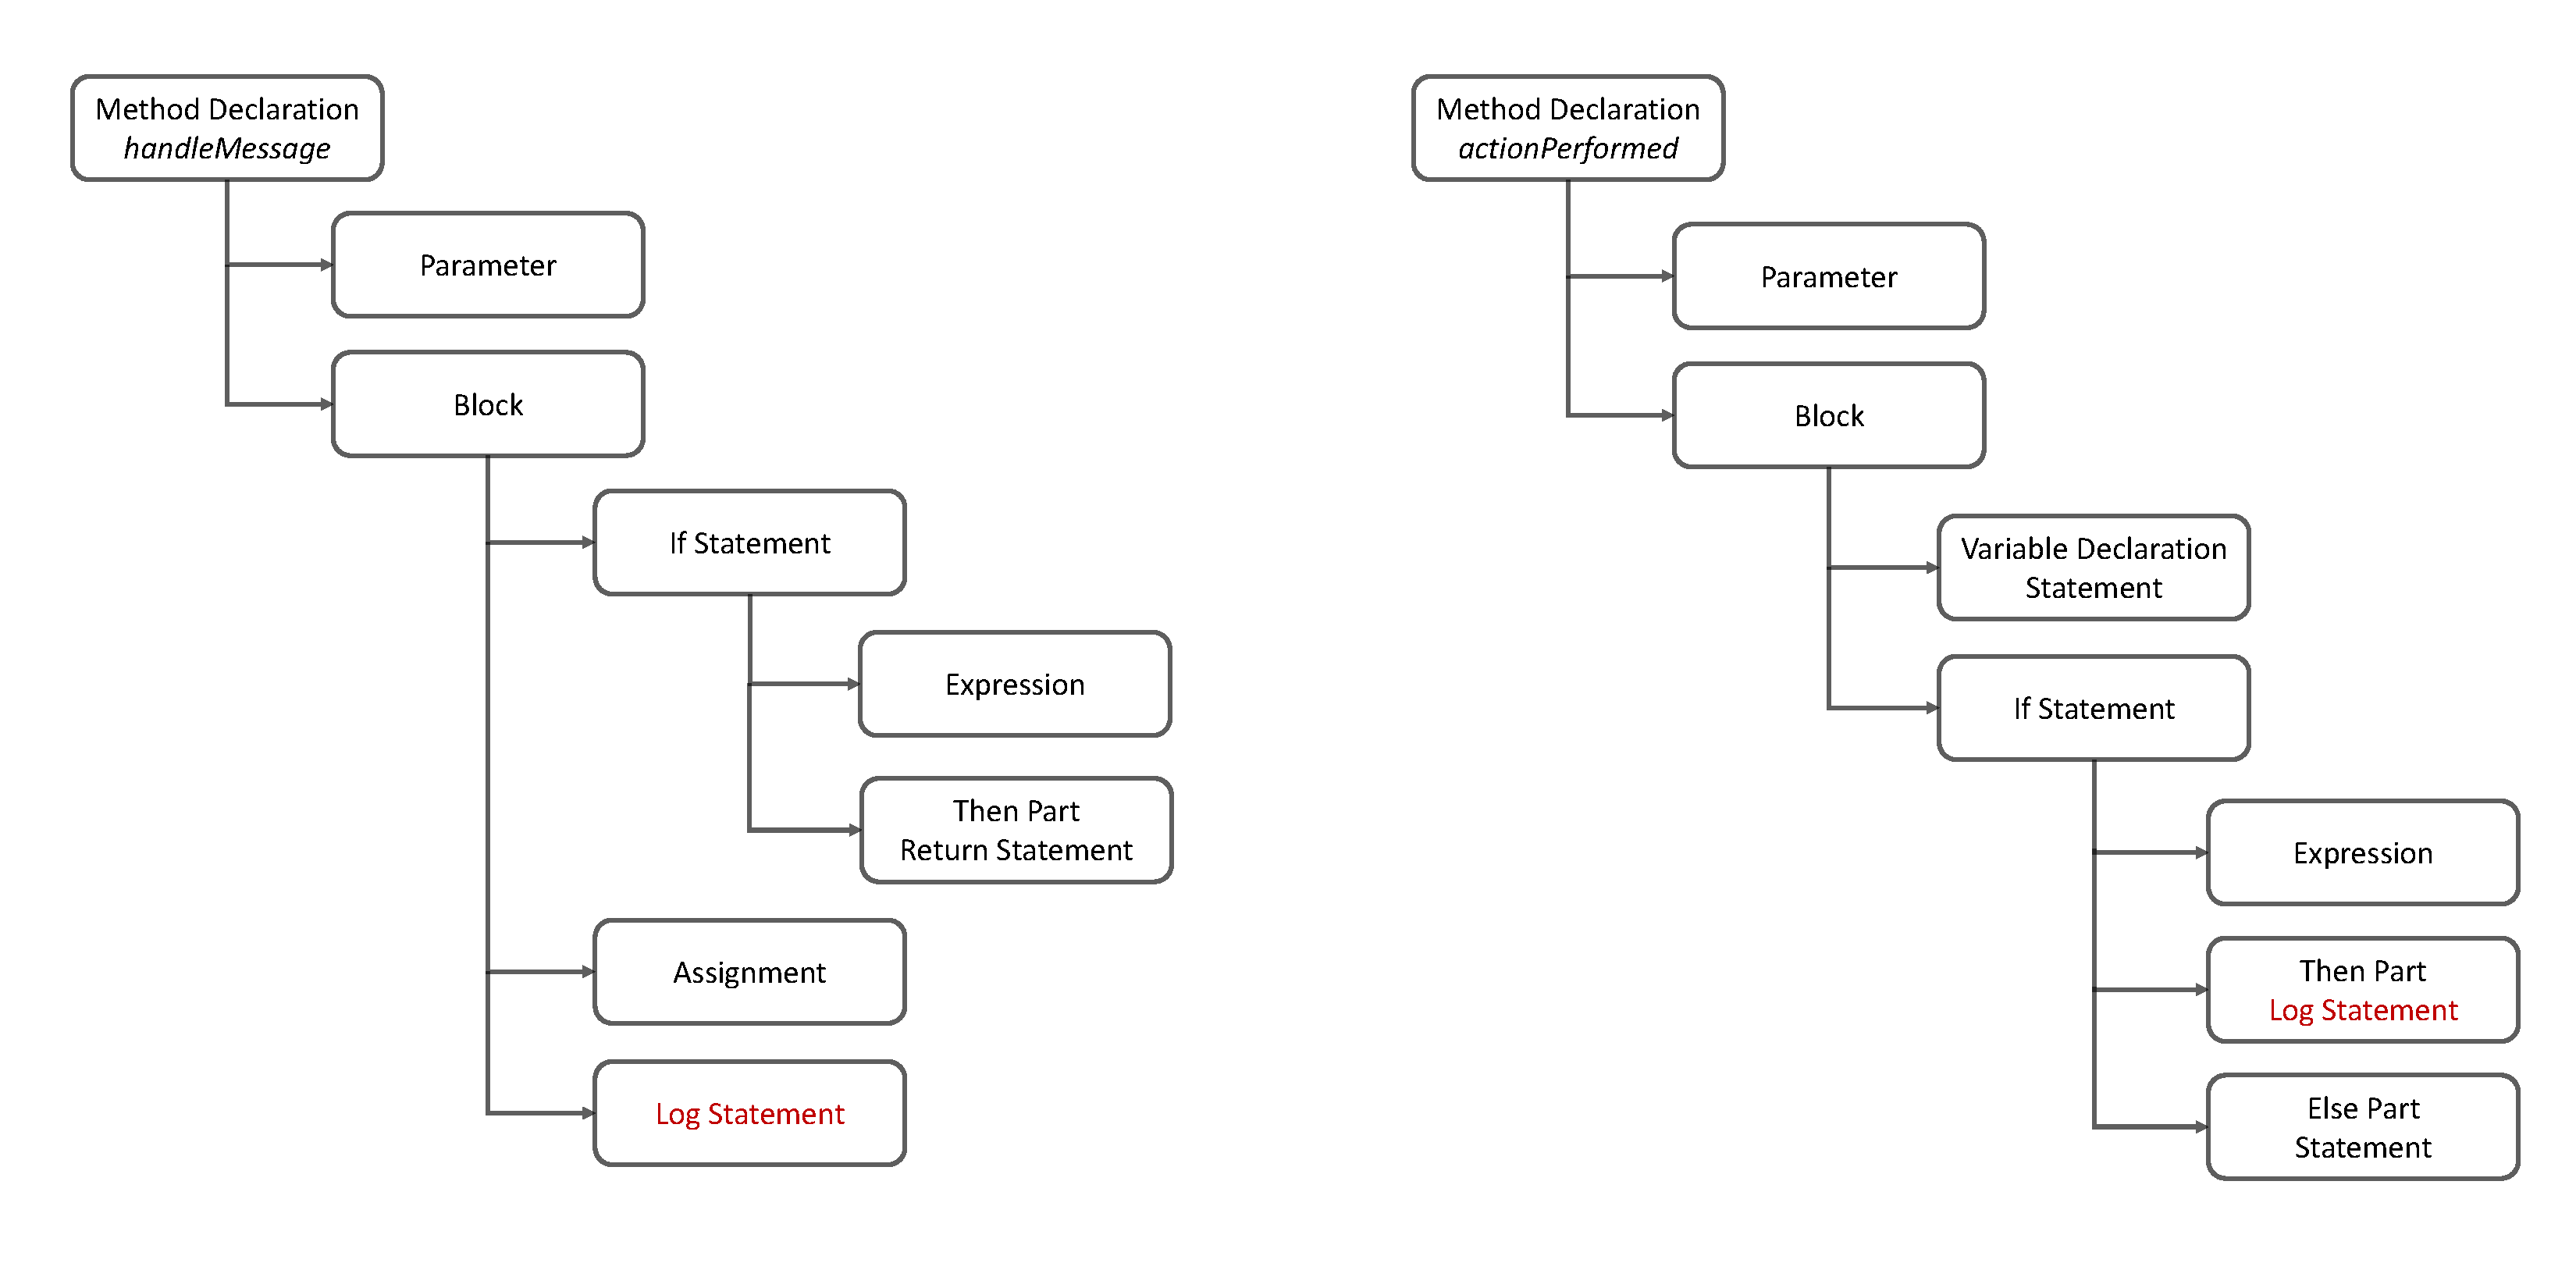
\includegraphics[width = \textwidth]{Drawing4/AST.pdf}
  \caption{Simple AST structure of the examples in Figures~\ref{ch3-ex1} and~\ref{ch3-ex2}.}
  \label{fig:ast}
\end{figure}

In the JDT framework, structural properties of each AST node can be used to obtain specific information about the Java element that it represents. These properties are stored in a map data structure that associates each property to its value; this data is divided into three types:
%property identifier???

\begin{itemize} [leftmargin=0.7in]
\item \textit{Simple structural properties:} These contain a simple value which has a primitive or simple type or a basic AST constant (e.g., identifier property of a name node whose value is a \code{String}).  For example, all the \textit{identifier} nodes in Figure~\ref{fig:java-example-ast} fall in this case; each references an instance of \code{String} representing the string that constitutes the identifier.
\item \textit{Child structural properties:} These involve situations where the value is a single AST node (e.g., name property of a method declaration node).  For example, the \textit{classDeclaration} node in Figure~\ref{fig:java-example-ast} has a single child that represents its name as an \textit{identifier} node.
\item \textit{Child list structural properties}: These involve situations where the value is a list of child nodes.  For example, the \textit{classDeclaration} node in Figure~\ref{fig:java-example-ast} can possess multiple \textit{modifier}s.
\end{itemize}

As an example, the ASTs of the log statements at line~4 of Figure~\ref{ch3-ex1} and Figure~\ref{ch3-ex2} can be represented respectively as:
\begin{itemize} [leftmargin=0.7in]
%\RW{These ASTs were messed up.  I fixed them according to what the code says.}
%\item \textit{expression(expression(Log), name(log), arguments(leftoperand(message), +, rightoperand(" is empty"), qualifier(Log), name(WARNING)))}
%\item \textit{expression(expression(Log), name(log), arguments(leftoperand(actionName),\\+, rightoperand("is an unknown action"), qualifier(Log), name(WARNING)))}
\item \textit{methodInvocation}(\\
\hspace*{1em}\textit{qualifiedName}(\code{Log}, \textit{identifier}(\code{log})),\\
\hspace*{1em}\textit{arguments}(\\
\hspace*{2em}\textit{qualifiedName}(\code{Log}, \mbox{\textit{identifier}(\code{WARNING})}),\\
\hspace*{2em}\textit{thisExpression}(),\\
\hspace*{2em}\textit{additionExpression}(\\
\hspace*{3em}\textit{methodInvocation}(\textit{identifier}(\code{getClassName}), \textit{arguments}()),\\
\hspace*{3em}\textit{stringLiteral}(\code{" should extend EditPlugin not EBPlugin since it has an empty "}),\\
\hspace*{3em}\textit{methodInvocation}(\textit{identifier}(\code{handleMessage}), \textit{arguments}()))))
\item \textit{methodInvocation}(\\
\hspace*{1em}\textit{qualifiedName}(\code{Log}, \textit{identifier}(\code{log})),\\
\hspace*{1em}\textit{arguments}(\\
\hspace*{2em}\textit{qualifiedName}(\code{Log}, \mbox{\textit{identifier}(\code{ERROR})}),\\
\hspace*{2em}\textit{thisExpression}(),\\
\hspace*{2em}\textit{additionExpression}(\\
\hspace*{3em}\textit{stringLiteral}(\code{"Unknown action: "}),\\
\hspace*{3em}\textit{identifier}(\code{actionName}))))
\end{itemize}

\section{First-order anti-unification}   \label{AU}

This section defines terms, substitutions, applying a substitution to a term, and instances of a term, as the requirements needed to describe first-order anti-unification.

\begin{defn}[First-Order Term]\label{def:term}
Given a set $V$ of variable symbols, a set $C$ of constant symbols, and sets $F_n$ of $n$-ary function symbols for all $n\ge1$, the set $T$ of \emph{first-order terms} is defined as the smallest set satisfying the recursion: (1) $V\subseteq T$; (2) $C\subseteq T$; and (3) for all $n$ first-order terms $t_1, \ldots, t_n$ and $n$-ary function symbol $f\in F_n$,  $f(t_1, \ldots, t_n) \in T$.
\end{defn}

Constant symbols can equivalently be considered 0-ary function symbols, with the appropriate adjustments to the above definition. For notational convenience, I use identifiers starting with a lowercase letter to represent function symbols (e.g., $f(a,b)$, $g(a,b)$) and constants (e.g., $a$, $b$), while variables are represented by identifiers starting with an uppercase letter (e.g., $X$, $Y$). The following are examples of a first-order term:
\begin{itemize} [leftmargin=0.7in]
\item $Y$
\item $a$
\item $f(X, c)$
\item $h(g(X, b),Y, g(a, Z))$
\end{itemize}
%A term is called grounded if it does not contain any variables (e.g., $f(a,b)}), and
Note that for any first-order term there is a unique, equivalent tree and vice versa: constant symbols and variable symbols are leaf nodes, while function symbols are non-leaf nodes; a function with given arguments is represented by a non-leaf node (representing the function symbol) with directed edges pointing to leaf nodes representing each argument.  For example:
\begin{itemize} [leftmargin=0.7in]
\item $Y$
\item $a$
\item \begin{tikzpicture}
\node(f) at (2,2) {$f$};
\node(X) at (1,1) {$X$};
\node(c) at (3,1) {$c$};
%
\draw[->](f) -- (X) {};
\draw[->](f) -- (c) {};
\end{tikzpicture}
%\item $X \leftarrow f \mapsto c$
\item \begin{tikzpicture}
\node(f) at (3,2) {$f$};
\node(g1) at (1,1) {$g$};
\node(Y) at (3,1) {$Y$};
\node(g2) at (5,1) {$g$};
\node(X) at (0,0) {$X$};
\node(b) at (2,0) {$b$};
\node(a) at (4,0) {$a$};
\node(Z) at (6,0) {$Z$};
%
\draw[->](f) -- (g1) {};
\draw[->](f) -- (Y) {};
\draw[->](f) -- (g2) {};
\draw[->](g1) -- (X) {};
\draw[->](g1) -- (b) {};
\draw[->](g2) -- (a) {};
\draw[->](g2) -- (Z) {};
\end{tikzpicture}
\end{itemize}

\begin{defn}[First-Order Substitution]\label{def:substitution}
A first-order substitution $\sigma$ is a mapping from variables $V$ to first-order terms $T$: $\sigma: V\mapsto T$. The notation $\{v_1 \mapsto t_1, \ldots, v_n \mapsto t_n\}$ is used to express a substitution of each of a set of variables $v_i$ by a corresponding first-order term $t_i$.
\end{defn}

\begin{defn}[Applying a First-Order Substitution]\label{def:substitution}
Applying a first-order substitution $\sigma = \{v_1 \mapsto t_1, \ldots, v_n \mapsto t_n\}$ to a first-order term $t$ results in the simultaneous replacement of all occurrences in $t$ of each variable $v_i$ by its corresponding first-order term $t_i$ as defined by the first-order substitution. This is denoted with the postfix expression $t\sigma$.
\end{defn}

As an example, applying the first-order substitution $\sigma = \{X \mapsto a, Y \mapsto b\}$
to the first-order term $f(X,Y)$ results in the replacement of all occurrences of the variable $X$ by the first-order term $a$ and all occurrences of the variable $Y$ by the first-order term $b$, and thus $f(X,Y)\sigma = f(a,b)$.

\begin{defn}[(First-Order) Instance]\label{def:instance}
For first-order terms $t_1$ and $t_2$, $t_2$ is called an \emph{instance} of $t_1$ if there exists a first-order substitution $\sigma$ such that $t_1\sigma = t_2$.
\end{defn}

%\begin{defn}[Unifier]\label{def:unifier}
%A unifier is a common instance of two given terms.
%\end{defn}

%Unification usually aims to create the \emph{most general unifier} (MGU); that is, $U$ is the MGU of two terms such that for all unifiers $U'$ there exists a substitution $\sigma$ such that $U\xrightarrow{\sigma}U'$. Unification aims to make a more concrete structure in essence, whereas what we need is a more generalized structure, which leads to the use of the dual of unification, called \emph{anti-unification}.

\begin{defn}[First-Order Anti-unifier]\label{def:generalization}
The term $t$ is a \emph{first-order anti-unifier} (or generalization) for first-order terms $t_1$ and $t_2$, if and only if there exist first-order substitutions $\sigma_1$ and $\sigma_2$ such that $t\sigma_1=t_1$ and $t\sigma_2=t_2$.
\end{defn}

A useful, first-order anti-unifier will contain only common pieces of the original terms, while the differences are abstracted away by replacing them with variable symbols. An anti-unifier for a pair of terms always exists since we can anti-unify any two terms by the term $X\in V$, i.e., a single variable. However, anti-unification usually aims to find the \emph{most specific anti-unifier} (MSA), that is, $t$ is the MSA of two first-order terms $t_1$ and $t_2$ if and only if there exists no anti-unifier $t'$ for $t_1$ and $t_2$ such that $t\sigma = t'$ for some first-order substitution $\sigma$.

As an example, an anti-unifier of the first-order terms $f(X,b)$ and $f(a,Y)$ is the first-order term $f(X,Y)$, containing common pieces of the two original, first-order terms. The variable $Y$ in the anti-unifier $f(X,Y)$ can be substituted by the first-order term $b$ to re-create $f(X,b)$ (with $\sigma_1 = \{Y\mapsto b\}$) and the variable $X$ in the anti-unifier can be substituted by the first-order term $a$ to re-create $f(a,Y)$
(with $\sigma_2 = \{X\mapsto a\}$), as depicted in Figure~\ref{fig:uni-anti-uni}.
%In addition, the unifier $f(a,b)$ of the two terms can be instantiated by applying the substitutions $\sigma_1'=X\xrightarrow{\sigma}a$ and $\sigma_2'=Y\xrightarrow{\sigma}b$ on the terms $f(X,b)$ and $f(a,Y)$, respectively.

\begin{figure} [t]
\centering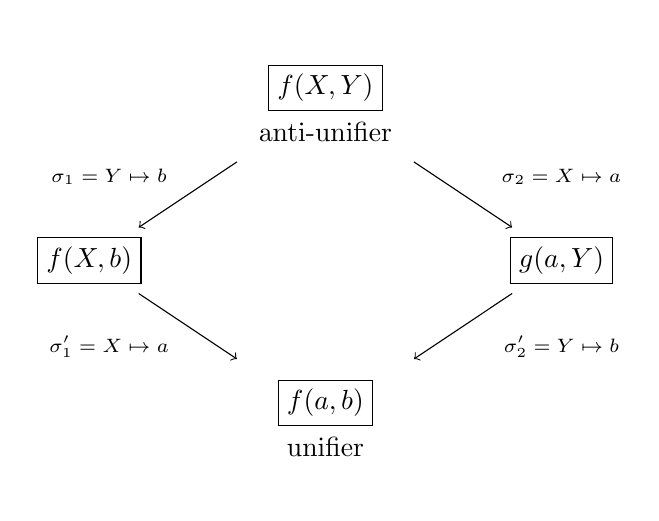
\begin{tikzpicture}
\node(au) at (5,2) {\parbox{2cm}{\begin{center}\fbox{$f(X,Y)$}\\*[3pt]\text{anti-unifier}\end{center}}};
\node(left) at (2,0) {\fbox{\mbox{$f(X,b)$}}};
\node(right) at (8,0) {\fbox{\mbox{$g(a,Y)$}}};
\node(u) at (5,-2) {\parbox{2cm}{\begin{center}\fbox{$f(a,b)$}\\*[3pt]\text{unifier}\end{center}}};
%
\draw[->](au) -- (left) node[pos=0.5, above]{\mbox{\scriptsize $\sigma_1 = Y \mapsto b$\hspace*{2cm}}};
\draw[->](au) -- (right) node[pos=0.5, above]{\mbox{\hspace*{2.5cm}\scriptsize $\sigma_2 = X \mapsto a$}};
\draw[->](left) -- (u) node[pos=0.5, below]{\mbox{\scriptsize $\sigma_1' = X \mapsto a$\hspace*{2cm}}};
\draw[->](right) -- (u) node[pos=0.5, below]{\mbox{\hspace*{2.5cm}\scriptsize $\sigma_2' = Y \mapsto b$}};
\end{tikzpicture}
%  {\makecell[l]{\hspace{0.4cm}f(X,Y)\\\text{anti-unifier}}}
%  \arrow{dr}{\sigma_2 = X \mapsto a}
%  \arrow[->,swap]{dl}{\sigma_1 = Y \mapsto b} % <-- reflect the direction of the hook
%\\
%f(X,b)
% \arrow[->,swap]{dr}{\sigma_1' = X \mapsto a}
% %\arrow{dr}
%&&
%f(a, Y)
%  \arrow{dl}{\sigma_2' = Y \mapsto b}
%  \\
%&
%{\makecell[l]{f(a,b)\\\text{unifier}}}
%\end{tikzcd}
%\]
  \caption{Unification and anti-unification of the terms $f(X,b)$ and $f(a,Y)$.}
  \label{fig:uni-anti-uni}
\end{figure}

The MSA should preserve as much of the common pieces of both original first-order terms as possible; however, first-order anti-unification fails to capture complex commonalities, as first-order substitutions only replace first-order variables by first-order terms. That is, when two first-order terms differ in function symbols, first-order anti-unification fails to retain common details of the arguments in both terms. For example, the first-order anti-unifier of the terms $f(a,b)$ and $g(a,b)$ is $X$ as depicted in Figure~\ref{fig:first-anti-uni}.

\begin{figure}[t]
\centering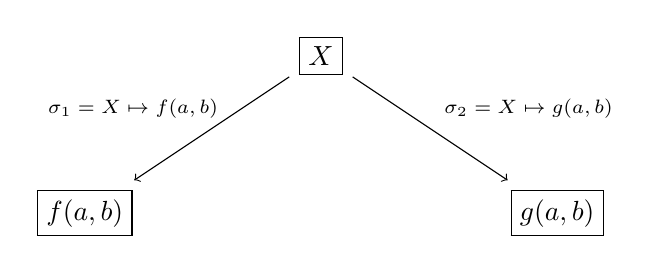
\begin{tikzpicture}
\node(au) at (5,2) {\fbox{\mbox{$X$}}};
\node(left) at (2,0) {\fbox{\mbox{$f(a,b)$}}};
\node(right) at (8,0) {\fbox{\mbox{$g(a,b)$}}};
%
\draw[->](au) -- (left) node[pos=0.5, above]{\mbox{\scriptsize $\sigma_1 = X \mapsto f(a,b)$\hspace*{2cm}}};
\draw[->](au) -- (right) node[pos=0.5, above]{\mbox{\hspace*{2.5cm}\scriptsize $\sigma_2 = X \mapsto g(a,b)$}};
\end{tikzpicture}
\caption{First-order anti-unification of the terms $f(a,b)$ and $g(a,b)$.\label{fig:first-anti-uni}}
\end{figure}

\subsection{Higher-order anti-unification}
 
Higher-order anti-unification generalizes first-order anti-unification to permit function symbols to be substituted for certain variable symbols (functional ones, to be precise).  The needed formal definitions follow.

\begin{defn}[Higher-Order Term]\label{def:hterm}
Given a set $V$ of variable symbols, a set $C$ of constant symbols, sets $F_n$ of $n$-ary function symbols for all $n\ge1$, and sets $\mathbf{V}_m$ of $m$-ary functional variable symbols, the set $\hat{T}$ of \emph{higher-order terms} is defined as the smallest set satisfying the recursion: (1) $V\subseteq \hat{T}$; (2) $C\subseteq \hat{T}$; (3) for all $n$ higher-order terms $\hat{t}_1, \ldots, \hat{t}_n$ and $n$-ary function symbol $f\in F_n$,  $f(\hat{t}_1, \ldots, \hat{t}_n) \in \hat{T}$; and (4) for all $m$ higher-order terms $\hat{t}_1, \ldots, \hat{t}_m$ and $m$-ary functional variable symbol $F\in \mathbf{V}_m$,  $F(\hat{t}_1, \ldots, \hat{t}_n) \in \hat{T}$.
\end{defn}
 
Note that any first-order term on $V$, $C$, and $F_n$ will also be (a degenerate case of) a higher-order term on $V$, $C$, $F_n$, and $\mathbf{V}_m$ for all $\mathbf{V}_m$.
 
\begin{defn}[Higher-Order Substitution]\label{def:substitution}
A higher-order substitution $\hat{\sigma}$ is a mapping from variables $V$ to higher-order terms $\hat{T}$: $\sigma: V\mapsto T$ and, for all natural numbers $m\ge1$, from $m$-ary functional variables $\mathbf{V}_m$ to $m$-ary functional symbols $F_m$. The notation $\{\hat{v}_1 \mapsto \hat{t}_1, \ldots, \hat{v}_n \mapsto \hat{t}_n\}$ is used to express a substitution of each of a set of variables and functional variables $\hat{v}_i$ by a corresponding higher-order term $\hat{t}_i$ or functional symbols, where it is to be understood that a $m$-ary functional variable may only be substituted by a $m$-ary functional symbol and that a variable may only be substituted by a higher-order term.
\end{defn}

Note that a first-order substitution constitutes (a degenerate case of) a higher-order substitution.

\begin{defn}[Applying a Higher-Order Substitution]\label{def:substitution}
Applying a higher-order substitution $\hat{\sigma} = \{\hat{v}_1 \mapsto \hat{t}_1, \ldots, \hat{v}_n \mapsto \hat{t}_n\}$ to a higher-order term $\hat{t}$ results in the simultaneous replacement of all occurrences in $\hat{t}$ of each variable (respectively functional variable) $\hat{v}_i$ by its corresponding higher-order term (respectively functional variable) $\hat{v}_i$ as defined by the higher-order substitution. This is denoted with the postfix expression $\hat{t}\hat{\sigma}$.
\end{defn}

As an example, a higher-order anti-unifier of the terms $f(a,b)$ and $g(a,b)$ is $F(a,b)$ as depicted in Figure~\ref{fig:higher-anti-uni}.   For simplicity, I henceforth drop the adjectival phrases ``first-order'' and ``higher-order'' in cases where the intent is clear from the context.

\begin{figure}[t]
\centering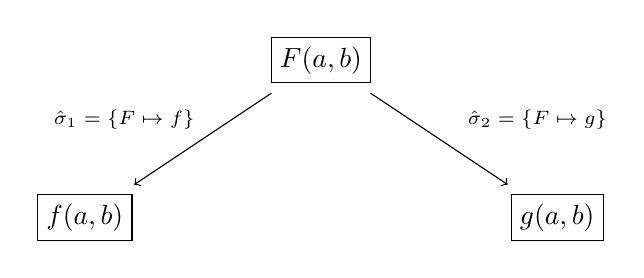
\begin{tikzpicture}
\node(au) at (5,2) {\fbox{\mbox{$F(a,b)$}}};
\node(left) at (2,0) {\fbox{\mbox{$f(a,b)$}}};
\node(right) at (8,0) {\fbox{\mbox{$g(a,b)$}}};
%
\draw[->](au) -- (left) node[pos=0.5, above]{\mbox{\scriptsize $\hat{\sigma}_1 = \{F \mapsto f\}$\hspace*{2cm}}};
\draw[->](au) -- (right) node[pos=0.5, above]{\mbox{\hspace*{2.5cm}\scriptsize $\hat{\sigma}_2 = \{F \mapsto g\}$}};
\end{tikzpicture}
\caption{A higher-order anti-unification of the terms $f(a,b)$ and $g(a,b)$.\label{fig:higher-anti-uni}}
\end{figure}

Applying higher-order anti-unification could help to construct a structural generalization by maintaining the common pieces and abstracting the differences away using variables. However, it is not comprehensive enough to solve the problem as it does not consider background knowledge about AST structures, such as syntactically different but semantically equivalent structures, missing structures, and different ordering of arguments.
%In the following section, we will look at an extension of anti-unification, higher-order anti-unification modulo theories, and how it can sufficiently address the limitations of anti-unification in our context.

\section{Neutral elements and pumping}

Sometimes it is desirable to anti-unify terms with differing numbers of arguments.  To permit this, we can utilize the notion of pumping transformations and neutral elements.  For example, with the binary function symbols ``$+$'' and ``$\times$'' we have the neutral elements ``0'' and ``1'' respectively, so that $+(x, 0)=x$ and $\times(x, 1)=x$ (also $+(0, x)=x$ and $\times(1, x)=x$ because of the commutativity of these functions).  We can generalize this notion to the special $n$-ary function symbols $\id{pump}_n$ and to the special constant symbols $\nu_{\id{pump}_n}$ (each representing the neutral symbol for the indicated function), so that for any term $t$,
\begin{equation*}
\id{pump}_n(\nu_{\id{pump}_n}, \ldots, \nu_{\id{pump}_n}, t, \nu_{\id{pump}_n}, \ldots, \nu_{\id{pump}_n}) = t,
\end{equation*}
where there are exactly $n$ arguments to $\id{pump}_n(\cdot)$.  Furthermore, we define $\id{pump}_n(\cdot)$ to be perfectly commutative, so that $t$ may equivalently appear as any argument therein.

For simplicity of exposition, we use the label \NIL{} in place of both the functional symbols $\id{pump}_n$ and the neutral element of each of the functions thereby defined, as the precise meaning can be interpreted from the context.  Obviously, \NIL{} representing an $n$-ary functional symbol cannot be meaningfully anti-unified with \NIL{} representing an $n-k$-ary functional symbol---unless it is itself pumped.

\section{Higher-order anti-unification modulo equational theories}\label{HOAUMT}

%\begin{align}
%\sigma_1 = (W &\mapsto \text{ \textsf{\small WARNING}},\nonumber\\
%X &\mapsto \text{ \textit{methodCall}(\textit{simpleName}(\textsf{\small getClassName}), \textit{arguments}())},\nonumber\\
%Y &\mapsto \text{ \textsf{\small "should extend EditPlugin not EBPlugin since it has an empty "}},\nonumber\\
%Z &\mapsto \text{ \textit{methodCall}(\textit{simpleName}(\textsf{\small handleMessage}), \textit{arguments}())})\label{eq:theta1}\\
%\sigma_2 = (W &\mapsto \text{ \textsf{\small ERROR}},\nonumber\\
%X &\mapsto \text{ \NIL{}},\nonumber\\
%Y &\mapsto \text{ \textsf{\small "Unknown action: "}},\nonumber\\
%Z &\mapsto \text{ \textit{simpleName}(\textsf{\small actionName})})\label{eq:theta2}
%\end{align}
%
%%\item it can be mapped to our recursive definition of a term, where AST nodes and simple values may be viewed as function-symbols and constants, respectively
%
%\begin{figure}[p]
%\begin{small}
%\begin{tikzpicture}
%\node(a) at (4.25,10) {%
%\fbox{\parbox[b][][b]{3in}{%
%\text{\textit{methodCall}(}\\
%\text{\hspace*{1em}\textit{qualifiedName}(\textsf{\footnotesize Log}, \textit{simpleName}(\textsf{\footnotesize log})),}\\
%\text{\hspace*{1em}\textit{arguments}(}\\
%\text{\hspace*{2em}\textit{qualifiedName}(\textsf{\footnotesize Log}, \textit{simpleName}(\textit{W})),}\\
%\text{\hspace*{2em}\textit{thisExpression}(),}\\
%\text{\hspace*{2em}\textit{additionExpression}(\textit{X}, \textit{stringLiteral}(\textit{Y}), \textit{Z})))}}}%
%};
%\node(b) at (0,0) {%
%\fbox{\parbox[t][][b]{3.1in}{%
%\text{\textit{methodCall}(}\\
%\text{\hspace*{1em}\textit{qualifiedName}(\textsf{\footnotesize Log}, \textit{simpleName}(\textsf{\footnotesize log})),}\\
%\text{\hspace*{1em}\textit{arguments}(}\\
%\text{\hspace*{2em}\textit{qualifiedName}(\textsf{\footnotesize Log},}\\ \text{\hspace*{3em}\mbox{\textit{simpleName}(\textsf{\footnotesize WARNING})}),}\\
%\text{\hspace*{2em}\textit{thisExpression}(),}\\
%\text{\hspace*{2em}\textit{additionExpression}(}\\
%\text{\hspace*{3em}\textit{methodCall}(\textit{simpleName}(\textsf{\footnotesize getClassName}),}\\ \text{\hspace*{4em}\textit{arguments}()),}\\
%\text{\hspace*{3em}\textit{stringLiteral}(\textsf{\footnotesize " should extend ... "}),}\\
%\text{\hspace*{3em}\textit{methodCall}(\textit{simpleName}(\textsf{\footnotesize handleMessage}),}\\ \text{\hspace*{4em}\textit{arguments}()))))}}}%
%};
%\node(c) at (8.5,0.7) {%
%\fbox{\parbox[t][][b]{2.55in}{%
%\text{\textit{methodCall}(}\\
%\text{\hspace*{1em}\textit{qualifiedName}(\textsf{\footnotesize Log}, \textit{simpleName}(\textsf{\footnotesize log})),}\\
%\text{\hspace*{1em}\textit{arguments}(}\\
%\text{\hspace*{2em}\textit{qualifiedName}(\textsf{\footnotesize Log},}\\ \text{\hspace*{3em}\mbox{\textit{simpleName}(\textsf{\footnotesize ERROR})}),}\\
%\text{\hspace*{2em}\textit{thisExpression}(),}\\
%\text{\hspace*{2em}\textit{additionExpression}(}\\
%\text{\hspace*{3em}\textit{stringLiteral}(\textsf{\footnotesize "Unknown action: "}),}\\
%\text{\hspace*{3em}\textit{simpleName}(\textsf{\footnotesize actionName}))))}}}%
%};
%
%\draw[->](a) -- (b) node[pos=0.5,above]{$\sigma_1\qquad$};
%\draw[->](a) -- (c) node[pos=0.5,above]{$\qquad\sigma_2$};
%\end{tikzpicture}
%\end{small}
%\caption{The anti-unification of the AUASTs of the logging calls in Examples 1 and 2.\label{fig:logging-anti}}
%\end{figure}
%%The AUASTs of log Method Invocation nodes from the Java classes in Figure~\ref{ch3-ex1} and Figure~\ref{ch3-ex2}.
%
%Applying higher-order anti-unification on AUAST structures could help to construct a structural generalization by maintaining the common pieces and abstracting the differences away using variables. However, it is not comprehensive enough to solve our problem as it does not consider background knowledge about AST structures, such as syntactically different but semantically relevant structures, missing structures, and different ordering of arguments. In the following section, we will look at an extension of anti-unification, higher-order anti-unification modulo theories, and how it can sufficiently address the limitations of anti-unification in our context.

%anti-unification cannot incorporate any background knowledge such as sematic knowledge required to solve our problem, and we should apply an extended form of anti-unification, called higher-order anti-unification modulo theories, where a set of equivalence equations is defined to incorporate semantic knowledge of structural equivalences supported by the Java language specification. An equivalence equation $=_E$ determines which terms are considered equal, and the set of equivalence equations must be applied on higher-order extended structures to allow the anti-unification of AST structures that are not identical but are semantically equivalent.
In higher-order anti-unification modulo (equational) theories, a set of equational theories, which treat different structures as equivalent, is defined to incorporate background knowledge. Each equational theory $=_E$ determines which terms are considered equal and a set of these equations can be applied on higher-order extended structures to determine structural equivalences. For example, we have introduced an equational theory $=_E$, such that $f(t,u) =_E f(u,t)$ to indicate that the ordering of arguments does not matter in our context.

% nil restriction!!!!
The notion of pumping from the previous section is equivalent to defining an equational theory $=_{\id{pump}}$ such that 
\begin{gather*}
\id{pump}_n(\nu_{\id{pump}_n}, \ldots, \nu_{\id{pump}_n}, t, \nu_{\id{pump}_n}, \ldots, \nu_{\id{pump}_n})\\
=_{\id{pump}} \id{pump}_{n-1}(\nu_{\id{pump}_{n-1}}, \ldots, \nu_{\id{pump}_{n-1}}, t, \nu_{\id{pump}_{n-1}}, \ldots, \nu_{\id{pump}_{n-1}})\\
=_{\id{pump}} \ldots\\
=_{\id{pump}} \id{pump}_1(t)\\
=_{\id{pump}} t
\end{gather*}
Or equivalently:
\begin{gather*}
\NIL{}(\NIL{}, \ldots, \NIL{}, t, \NIL{}, \ldots, \NIL{})\\
=_{\id{pump}} \NIL{}(\NIL{}, \ldots, \NIL{}, t, \NIL{}, \ldots, \NIL{})\\
=_{\id{pump}} \ldots\\
=_{\id{pump}} \NIL{}(t)\\
=_{\id{pump}} t
\end{gather*}
For simplicity, I refer to this as the \NIL{}-theory. 

For example, we can anti-unify the two terms $b$ and $f(a,b)$ through the application of the \NIL{}-theory by creating the term $\NIL{}(\NIL{},b)$---which is $=_{\id{pump}}$ to $b$---and anti-unifying $\NIL{}(\NIL{},b)$ with $f(a,b)$ as depicted in Figure~\ref{fig:anti-nil} to arrive at $F(X, b)$.

%restrictions???

% to introduce an equivalence equation =E for the NIL structure
% it should be modified
% should it be different?
\begin{figure}[t]
\centering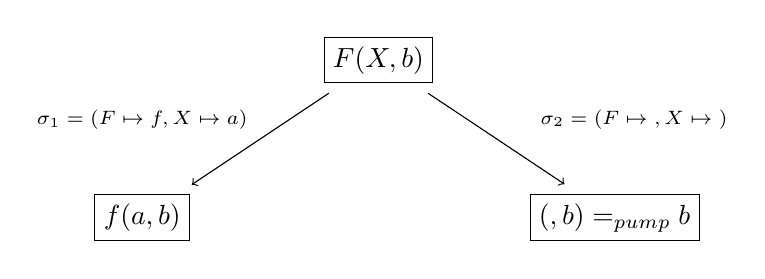
\begin{tikzpicture}
\node(au) at (5,2) {\fbox{\mbox{$F(X,b)$}}};
\node(left) at (2,0) {\fbox{\mbox{$f(a,b)$}}};
\node(right) at (8,0) {\fbox{\mbox{$\NIL{}(\NIL{},b) =_{\id{pump}}  b$}}};
%
\draw[->](au) -- (left) node[pos=0.5, above]{\mbox{\scriptsize $\sigma_1 = ( F \mapsto f, X \mapsto a)$\hspace*{3cm}}};
\draw[->](au) -- (right) node[pos=0.5, above]{\mbox{\hspace*{3.5cm}\scriptsize $\sigma_2 = ( F \mapsto \NIL{}, X \mapsto \NIL{})$}};
\end{tikzpicture}
\caption{Higher-order anti-unification modulo theories of the terms $f(a, b)$ and $b$.\label{fig:anti-nil}}
\end{figure}


We have also defined a set of equational theories to incorporate semantic knowledge of structural equivalences supported by the \name{Java} language specification, as it provides various syntactic ways to define semantically equivalent structures. 
%These theories should be applied on higher-order extended structures to anti-unify AST structures that are not identical but are semantically equivalent. 
For example, consider \code{for}- and \code{while}-statements that are two kinds of looping structure in \name{Java}: they have different syntax but cover the same concept. To be able to anti-unify these structures meaningfully, we need an equational theory that can equate any \code{for}-loop---\code{for(}$\id{inits}$\code{; }$\id{test}$\code{; }$\id{updates}$\code/){...}/---to an equivalent \code{while}-loop---$\id{inits}$\code{; while(}$\id{test}$\code/) {...; /$\id{updates}$\code/;}/.  


Most simply, we could treat the two loops as functions with differing arguments, defining an equivalence equation $=_{\id{loops}}$ that allows their direct anti-unification. We would then utilize the \NIL{}-theory to handle the varying number of arguments as the \code{for}-loop has three arguments whereas the \code{while}-loop only has one. Using the \NIL{}-theory we can create the structure \code{while}(\NIL{}(\NIL{}, \NIL{}), \textit{lessThanExpression}(\code{i}, \code{10}), \NIL{}(\NIL{}, \NIL{})) that is $=_{\id{loops}}$ to \code{while}(\textit{lessThanExpression}(\code{i}, \code{10})) and construct the anti-unifier, $V_0$($V_1$($V_2$, $V_3$), \textit{lessThanExpression}(\code{i}, \code{10}), $V_4$($V_5$($V_2$))), as depicted in Figure~\ref{fig:for-while}.

\begin{figure}[t]
\centering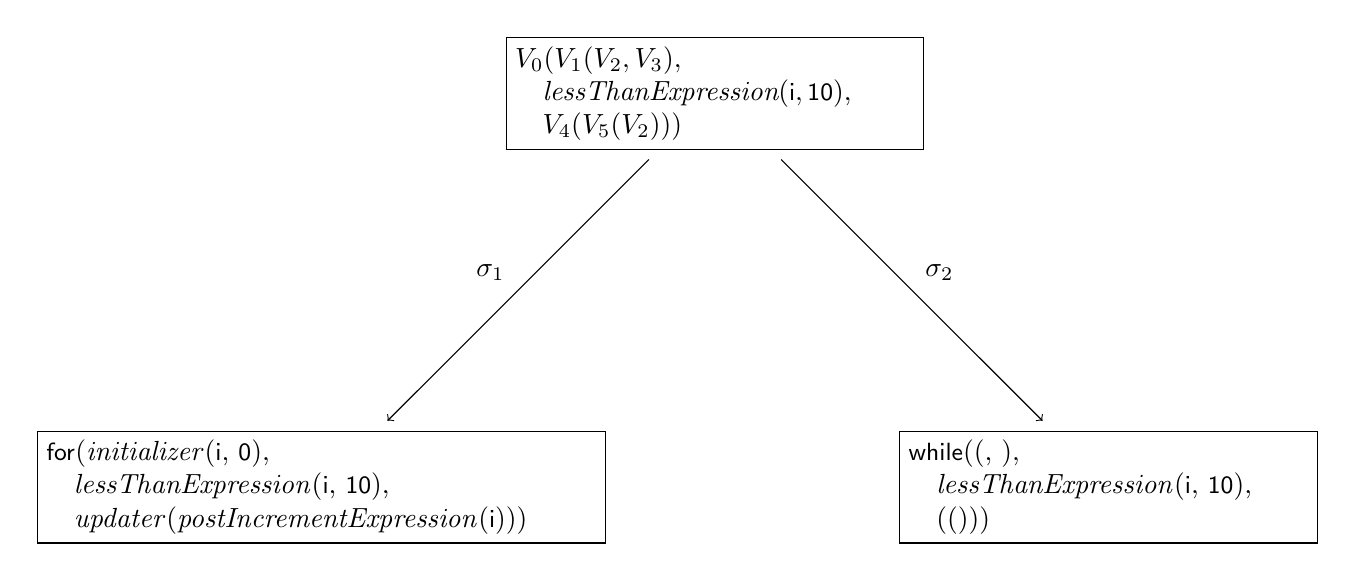
\begin{tikzpicture}
\node(au) at (5,5) {\fbox{\parbox{2in}{$V_0(V_1(V_2,V_3),$\\$\text{\quad\textit{lessThanExpression}(\textsf{\small i}, \textsf{\small 10})}$,\\ \mbox{$\quad V_4(V_5(V_2)))$}}}};
%
\node(left) at (0,0) {\fbox{\parbox{2.75in}{%
\textsf{\small for}(\textit{initializer}(\textsf{\small i}, \textsf{\small 0}),\\\mbox{\quad\textit{lessThanExpression}}(\textsf{\small i}, \textsf{\small 10}),\\ \mbox{\quad\textit{updater}}(\textit{postIncrementExpression}(\textsf{\small i})))}}};
%
\node(right) at (10,0) {\fbox{\parbox{2in}{%
\textsf{\small while}(\NIL{}(\NIL{}, \NIL{}),\\ \mbox{\quad\textit{lessThanExpression}}(\textsf{\small i}, \textsf{\small 10}),\\ \mbox{\quad\NIL{}}(\NIL{}(\NIL{})))}}};
%
\draw[->](au) -- (right) node[pos=0.5, above]{$\qquad\sigma_2$};
%
\draw[->](au) -- (left) node[pos=0.5, above]{$\sigma_1\qquad$};
\end{tikzpicture}
\caption[Complex anti-unification of two structures demonstrating a \protect\NIL{}-theory.]{Anti-unification of the structures \code{for}(\textit{initializer}(\code{i}, \code{0}), \mbox{\textit{lessThanExpression}(\code{i}, \code{10}),} \textit{updater}(\textit{postIncrementExpression}(\code{i}))) and \code{while}(\NIL{}(\NIL{}, \NIL{}), \mbox{\textit{lessThanExpression}(\code{i}, \code{10}),} \NIL{}(\NIL{}, \NIL{})). The substitutions are defined as follows: $\sigma_1 = (V_0 \mapsto \text{ \textsf{\small for}}, V_1 \mapsto \text{ \textit{initializer}}, V_2 \mapsto \text{ \textsf{\small i}}, V_3 \mapsto 0, V_4 \mapsto \text{ \textit{updater}}, V_5 \mapsto \text{ \textit{postIncrementExpression}})$; and $\sigma_2 = (V_0 \mapsto \text{ \textsf{\small while}}, V_1 \mapsto \text{ \NIL{}}, V_2 \mapsto \text{ \NIL{}}, V_3 \mapsto \text{ \NIL{}}, V_4 \mapsto \text{ \NIL{}}, V_5 \mapsto \text{ \NIL{}})$\label{fig:for-while}}
\end{figure}
% higher-order extension and the equational theories
% provide a better example

In practice, this is more usefully accomplished by converting the \code{for}-loop to the equivalent \code{while}-loop and anti-unifying the result directly, which can find correspondences between the initialization expression and equivalent assignment statements prior to the \code{while}-loop, and between the update expression and equivalent statements, typically at the end of the block in the \code{while}-loop.

\subsection{Loss of uniqueness}
Defining complex substitutions in higher-order anti-unification modulo theories results in losing the uniqueness of the MSA. For example, consider the terms $f_1(g(a,e))$ and $f_2(g(a,b),$\linebreak$g(d,e))$. As described in Figure~\ref{fig:multipleMSA}, two MSAs exist for these terms: we can anti-unify $g(a,e)$ and $g(a,b)$ to create the anti-unifier $g(a,X_0)$ and anti-unify $g(d,e)$ with the \NIL{} structure to create the anti-unifier $G(Z,X_1)$; or we can anti-unify $g(a,e)$ and $g(d,e)$ to create the anti-unifier $g(X_0,e)$ and anti-unify $g(a,b)$ with the \NIL{} structure to create the anti-unifier $F(Z,X_1)$.

\begin{figure}[t]
\centering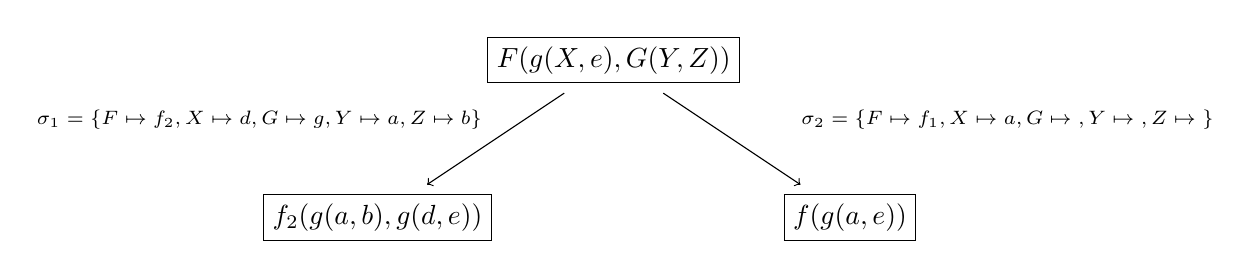
\begin{tikzpicture}
\node(au) at (5,2) {\fbox{\mbox{$F(g(X,e),G(Y,Z))$}}};
\node(left) at (2,0) {\fbox{\mbox{$f_2(g(a,b), g(d,e))$}}};
\node(right) at (8,0) {\fbox{\mbox{$f(g(a,e))$}}};
%
\draw[->](au) -- (left) node[pos=0.5, above]{\mbox{\scriptsize $\sigma_1 = \{F\mapsto f_2, X\mapsto d, G\mapsto g, Y\mapsto a, Z\mapsto b\}$\hspace*{6cm}}};
\draw[->](au) -- (right) node[pos=0.5, above]{\mbox{\hspace*{7cm}\scriptsize $\sigma_2 = \{F\mapsto f_1, X\mapsto a, G\mapsto \NIL{}, Y\mapsto \NIL{}, Z\mapsto \NIL{}\}$}};
\end{tikzpicture}
\vspace*{1em}

\centering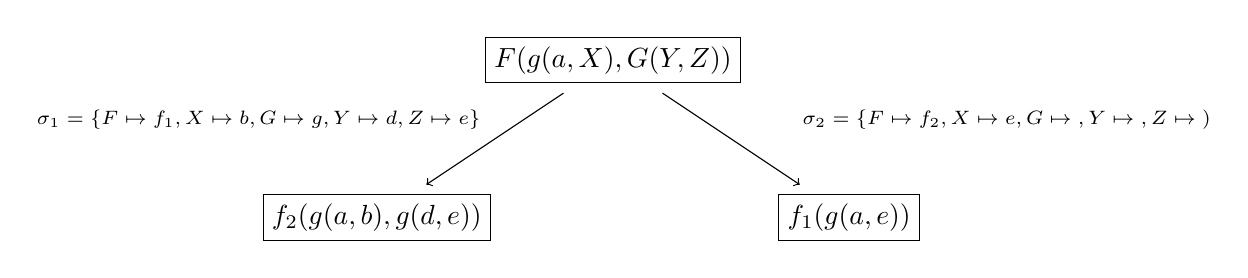
\begin{tikzpicture}
\node(au) at (5,2) {\fbox{\mbox{$F(g(a,X),G(Y,Z))$}}};
\node(left) at (2,0) {\fbox{\mbox{$f_2(g(a,b), g(d,e))$}}};
\node(right) at (8,0) {\fbox{\mbox{$f_1(g(a,e))$}}};
%
\draw[->](au) -- (left) node[pos=0.5, above]{\mbox{\scriptsize $\sigma_1 = \{F\mapsto f_1, X\mapsto b, G\mapsto g, Y\mapsto d, Z\mapsto e\}$\hspace*{6cm}}};
\draw[->](au) -- (right) node[pos=0.5, above]{\mbox{\hspace*{7cm}\scriptsize $\sigma_2 = \{F\mapsto f_2, X\mapsto e, G\mapsto\NIL{}, Y\mapsto\NIL{}, Z\mapsto\NIL{})$}};
\end{tikzpicture}
\caption[Ambiguous higher-order anti-unification modulo theories of two terms.]{Ambiguous higher-order anti-unification modulo theories of the terms $f_2(g(a,b), g(d,e))$
and $f_1(g(a,e))$, creating multiple MSAs.}
  \label{fig:multipleMSA}
\end{figure}


Despite having multiple potential MSAs, I need to determine one single MSA that is the most appropriate in my context. However, the complexity of finding an optimal MSA is undecidable in general \cite{2008:fse:cottrell} since an infinite number of possible substitutions can be applied to variables in a term. Therefore, I need to use an approximation technique to construct one of the best MSAs that can sufficiently solve the problem.
% reason, infinite number??? ever variable???
%Our goal is to find an MSA that is an approximation of the best fit to our application


\section{The Jigsaw Tool}\label{Jigsaw}

\name{Jigsaw} is a plug-in to the Eclipse integrated development environment (IDE), which was developed by \citet{2008:fse:cottrell} to support small-scale source code reuse via structural correspondence. A small-scale reuse task can be divided into two phases. The first phase involves the developer identifying a source code snippet that implements functionality that is missing within a target system. The second phase involves integrating the source code snippet within the target system.
\name{Jigsaw} supports the small scale reuse task by identifying structural correspondences between the code snippet and the context into which the code should be pasted, in order to suggest to developers what parts already exist within the target system, what parts are missing, and what parts need to be modified to fit into the context. In summary, the \name{Jigsaw} tool determines the structural correspondences between two \name{Java} source code fragments through the application of higher-order anti-unification modulo equational theories such that one fragment can be integrated to the other one for small-scale code reuse.

%To perform a reuse task, developers mostly copy and paste the reused code snippet and then fit it to the hole of the target context by performing some modifications.

In general, the proposed approach by \citeauthor{2008:fse:cottrell} proceeds in three steps. First, it generates an augmented form of AST, called a \emph{correspondence AST} (CAST), where each node holds a list of candidate correspondence connections, each implicitly representing an anti-unifier. To find candidate correspondences amongst the CASTs of the original system and the target system, it uses a similarity measure that relies on syntactic similarity along with simple knowledge of semantic equivalences supported the Java language specifications. Although the CAST structure may represent many anti-unifiers, they used a greedy selection algorithm to select the best fit for each node via thresholding in order to approximate the optimal generalization. That is, the correspondence connections with a similarity value below a threshold are removed. Second, when there is more than one candidate correspondence connection for a node, the developer is prompted to resolve the conflict by selecting the best fit for his functionality. Third, the best correspondences are used to semi-automatically perform the integration task by replacing the references to variables in the original system by the references to variables in the target system. The Jigsaw tool is a proof-of-concept implementation of this approach.

Underlying the Jigsaw tool is the Jigsaw framework for determining likely structural correspondences between two ASTs; I simply refer to ``Jigsaw'' henceforth to intend the Jigsaw framework.
The Jigsaw similarity function returns a value in $[0, 1]$ where zero indicates complete lack of similarity and one indicates perfect similarity. In general, this function returns a value above zero if the compared nodes are of identical type, and thus it returns a similarity of 0 for the nodes of different types. However, it uses several heuristics to improve the utility of the similarity measurement by defining an arbitrary value for the nodes that are syntactically different but are semantically relevant. For example, the similarity between names of AST nodes is measured using a normalized computation based on the length of the longest common substring. The comparison of the \code{int} and \code{long} nodes is another example, where an arbitrary value of 0.5 is defined as the similarity, since they are not of syntactically identical types but have a semantic equivalence. This function also detects the correspondence between \code{for}-, \code{enhanced-for}-, \code{while}-, and \code{do}-loop statements; and \code{if} and \code{switch} conditional statements.


As I intend to construct a structural generalization from ASTs of two logged methods via structural correspondence, it could be helpful to use the first phase of the proposed approach to find candidate correspondences using the similarity measure. However, the second phase does not help determine the best correspondences needed in my context, as the CAST generated via thresholding neither resolves the conflicts that occur in constructing one single anti-unifier automatically, nor prevents the anti-unification of log statement nodes with any other nodes. There, the Jigsaw similarity function does not enable us to measure how similar are the usages of log statements inside methods. In addition, as the problem of this study is different, the integration phase of the approach is not related to my work. Instead, I should develop an algorithm to construct a detailed view of the generalization describing the structural commonalities and differences between logged methods. However, the CAST structure does not suffice to construct an anti-unifier: it does not allow the insertion of \emph{structural variables} in place of nodes in the tree structure, and thus an extended form is required. In the following chapters, I will discuss my approach to create a structural generalization and its implementation by means of the higher-order anti-unification modulo theories.
\section{Clustering}  \label{ch3-clustering}
Clustering is the classification of a collection of data objects into meaningful groups (clusters) \cite{jain1999data}. The goal of clustering is to find groups of objects such that the objects in one cluster will be similar to one another and dissimilar from the objects in other clusters. The greater the similarity amongst the objects within a cluster and the greater the dissimilarity between the objects from various clusters are, the more distinct the clusters would be \cite{}.  In general, there are two major types of clustering:
%\cite[][Chapter 8]{tan2013data} ????

\begin{itemize} [leftmargin=.4in]
\item \emph{Partitional clustering:} which aims to divide the data objects into non-overlapping clusters such that each data object is in utterly one cluster.
\item \emph{Hierarchical clustering:} which aims to generate a set of nested clusters organized as a hierarchical structure. Each cluster in the structure is the union of its subclusters, and the cluster at the top contains all the the data objects.
\end{itemize}

The following will introduce two popular techniques used to perform clustering on a data set:

% supervised-unsupervisod?
%dendogram?
\subsubsection{K-means clustering algorithm}
% indicate Lines ??? initial centroids???
This algorithm is a partitional clustering approach that attempts to find a certain number of clusters, which are represented by centriod (the center of a cluster). In this algorithm, ${K}$ is the number of the resulting clusters that should be specified. Each cluster is associated with a centroid  which is mostly the average of all the
data objects within the cluster or the most representative object of a
cluster. The basic K-means clustering technique is described using the Algorithm~\ref{alg:k-means}. This algorithm repeatedly assigns each data object to a cluster with the nearest centroid and computes the new clusters centroids accordingly. This process terminates when it reaches a state in which no objects are moving from one cluster to another, and thus, the centroids don't change.
%strength?
The K-means clustering algorithm is not a good fit to this study, as it requires to specify the number of resulting clusters, which is not reasonable to my problem context. %??
% representative object?

%Each object is assigned to a centroid is a cluster. The centroid of each cluster is then updated based on the objects assigned to the cluster.  repeatedly perform the assignment and update opertaions util the centroids do not change.

\begin{algorithm}
\caption{Basic K-means clustering algorithm.} \label{alg:k-means}
\begin{algorithmic}[1]
\State Select K data objects as initial centroids.
\Repeat
\State Assigning each object to its closes centroid.
\State Update the centroid of each cluster.
\Until Centroids remain the same.
\end{algorithmic}
\end{algorithm}



\subsubsection{Agglomerative hierarchical clustering algorithm}
%LINES???
%dendogram?
The agglomerative hierarchical clustering algorithm produce a nested grouping of clusters, with single point clusters at the bottom and an all-inclusive cluster at the top \cite{karypis1999chameleon}. Agglomerative hierarchical clustering is one of the main stream clustering methods \cite{day1984efficient} that has applications in document retrieval \cite{voorhees1986implementing} and information retrieval from a search engine query log \cite{beeferman2000agglomerative}. Algorithm~\ref{alg:agglomerative} describes the basic agglomerative hierarchical clustering appraoch. It starts with the individual objects as singleton clusters, and successively, merges the two closest clusters until only one all inclusive cluster remains. In general, hierarchical clustering algorithms work implicitly or explicitly with the $n \times n$ similarity matrix such that an element in row $i$ and column $j$ represents the similarity between the $i$th and the $j$th clusters \cite{karypis1999chameleon}.
% dandogram ???
%update???


\begin{algorithm}
\caption{Basic agglomerative hierarchical clustering algorithm.} \label{alg:agglomerative}
\begin{algorithmic}[1]
\State Start with singleton clusters.
\State Compute the similarity matrix.
\Repeat
\State Merge the closest cluster pair.
\State Update the similarity matrix by computing the similarity between new cluster and all remaining clusters.
\Until Only one cluster remains.
\end{algorithmic}
\end{algorithm}




%until a pre-determined number of clusters is obtained or the similarity between the closest clusters becomes below a pre-determined threshold value.

%[Rasmussen, 1992] \RW{Put into bibtex}?????

There are various versions of agglomerative hierarchical algorithms that mainly differ in how they update the similarity between clusters. There are various methods to measure the similarity between clusters, such as single linkage, complete linkage, average linkage, and centroids \cite{}. In the single linkage method, the similarity is measured by the similarity of the closest pair of data points of two clusters. In the complete linkage method, the similarity is computed by the similarity of the farthest pair of data points of two clusters. In the average linkage method, the similarity is measured by the average of all pairwise similarities between data points of two clusters. In the centroids methods, each cluster is represented by a centroid, and the similarity between two clusters is measured by the similarity of the clusters' centroids. However, I need to develop a modified version of the basic agglomerative hierarchical clustering algorithm to address my problem context. In the modified version, the merge and update operations should be terminated when the similarity between the closest clusters becomes below a pre-determined threshold value. Furthermore, I need to develop a measure of the similarity between the clusters based on the similarity between their anti-unifiers. In Chapter~\ref{clustering}, I describe how I modified the basic hierarchical algorithm to my problem context.

%in our application, each cluster is composed of one AUAST, and the similarity between two clusters is measured by the similarity between the clusters' AUASTs, which is the ratio of the number of common pieces over the total number of pieces of their anti-unifier.


%optimal clusters
%. Partitional clustering try to classify a data set into $k$ clusters such that the partition optimizes a pre-determined criterion \cite{karypis1999chameleon}. The most popular partitional clustering algorithm is $k$-means, which repeatedly assigns each data point to a cluster with the nearest centroid and computes the new cluster centroids accordingly until a pre-determined number of clusters is obtained \cite{bouguettaya2015efficient}.

\section{Summary}  \label{summary}
I described abstract syntax trees (ASTs) as a standard syntactic representation of source code. Every AST can also be represented in a functional format (and vice versa) which constitute the standard theoretical concept of terms. I presented Eclipse JDT as a concrete framework that can be used to manipulate ASTs of a source code written in the \name{Java} programming language.

I demonstrated how the theoretical framework of anti-unification can be used as a technique to construct a common generalization of two given terms, and hence of two ASTs.  First-order anti-unification permits terms to be replaced with variables and vice versa, but it is limited in that low-level commonality can be discarded due to high-level differences.  Higher-order anti-unification overcomes this by permitting substitution relative to function symbols as well as terms. A further extension allows for insertion and deletion by declaring equivalence with the \NIL{} structure, as well as other arbitrary equational theories to embed knowledge of semantic equivalence.  Unfortunately, this approach of higher-order anti-unification modulo theories leads to ambiguity and the potential for an infinite number of possible substitutions for every structural variable.  To make use of that technique despite its weaknesses, we must apply an approximation technique to select amongst the best MSAs in order to reach a solution that is reasonable in practice. I also introduced Jigsaw, an existing framework for determining structural correspondences between ASTs and why it does not adequately address my problem.  To address my problem, I describe in subsequent chapters how I extended the Jigsaw framework. Furthermore, I introduced a hierarchical clustering algorithm that can be applied to classify logged methods into different categories.

%approximated or modified? 